\section{\hostapi{} efficiency}


The efficiency of \hostapis{} directly impacts the performance of \graphene{} on each host.
A large portion of \linuxapis{} inside \thelibos{} require resources or abstractions from the host OS.
Since \thehostabi{} is the only interface for requesting host OS features,
the definition of \thehostabi{}
restricts the options for a \picoproc{} to optimize its own performance, according to the application's performance patterns.
Although each PAL may optimize individual \hostapi{} for general circumstances,
all applications must share the same PAL ABI and thus tolerate the same overheads of exporting these \hostapis{} on each host.




Three primary factors determine the efficiency of \hostapis{}.
First, especially on Linux or other monolithic OS,
most of \thehostabi{} are directly translated to similar \linuxapis{}.
The efficiency of these \hostapis{}
are dominated by the basic cost of the host system interface,
and the performance of corresponding \linuxapis{}.
For instance, on a Linux host, \palcall{StreamRead} is directly translated to \syscall{pread}, and thus might show similar latency as the \linuxapi{} without further security checks. 
If \graphene{} runs inside an SGX enclave,
the \hostapis{} is further panelized with additional overheads that contribute to exiting the enclave for host system calls, and bringing memory into the EPC (enclave page cache) or decrypting 
memory on a last-level cache miss.


The second factor is the translation cost
of the \hostapis{}.
For portability, \thehostabi{} is defined with generic semantics, without host-specific notions
such as process identifiers, file descriptors,
file system paths,
and \linuxapi{} flags.
The PAL must translate the arguments of \hostapis{}, including PAL handles, URIs (Uniform Resource Identifiers), and generic flags,
to the arguments interpretable by the host kernel.
 


Finally, the third factor that impacts the PAL call efficiency
is the cost of security checks,
either inside the host kernel or the guest.
The cost of security checks varies between hosts, and is correlated with the presumed security models.
On a regular Linux host, the security model
focuses on isolating mutually-untrusting applications,
therefore requires checking
the \hostapis{} in the Linux kernel,
to restrict the sharing of host resources and unpermitted system interfaces,
using both the reference monitor and SECCOMP filter.
Inside an SGX enclave, the security checks
for the \hostapis{}
protects the application and \libos{} from an untrusted OS,
and thus focus on validating the results of \linuxapis{},
using either cryptographic techniques or semantic checks.
Cryptographic techniques are used to: (1) validate the file against the secure hash, at \palcall{StreamOpen}, (2) check the file chunks against a Merkle tree of hash values, at \palcall{StreamRead}, and (3) establish a TLS connection over inter-enclave RPC, at \palcall{ProcessCreate}.
The evaluation shows
that the cost of security checks
may dominate the latency of \hostapis{} on a host like SGX. 


This section evaluates the efficiency of \hostapis{} on both Linux and SGX hosts, and shows the impact of each performance factor.
The evaluation is based on micro-benchmark programs similar to \lmbench{} 2.5~\cite{McVoy:lmbench},
and is compared against
similar \linuxapis{} on Linux.



\subsection{Stream I/O}


The \hostapis{} for stream I/O can be separated into two types of operations:
file system operations and I/O operations on a network socket or a RPC stream.
The file system operations
access a UNIX-style, hierarchical, host file system,
with either random access to file contents,
or access to file attributes (metadata).
The I/O operations on a network socket or a RPC stream
allow sending and receiving sequential messages over a network address or a local, in-kernel queue.
Due to the difference in the nature of these operations,
the evaluation separates
file access from network or RPC workloads.




\paragraph{Opening a file.}
Figure~\ref{fig:eval:pal:open-latency} (a) shows the latency of \palcall{StreamOpen} on a Linux PAL, versus the latency of \syscall{open} \linuxapis{} in a native Linux process.
The latency of \syscall{open} \linuxapis{} on Linux is correlated with
the lengths and depths of opened file paths,
due to the design of file system directory cache
in the Linux kernel~\cite{tsai15dcache}.
The Linux kernel searches the metadata of a file path queried by \syscall{open} or \syscall{stat}, by looking up the path components (i.e., directory names separated by the common slash character)
inside the file system directory cache.
Because the Linux PAL only implements \palcall{StreamOpen} using \syscall{open}, the latency of \palcall{StreamOpen} is similar to \syscall{open} with a small overhead around 6--10\% for
scanning the file URI and translating other \linuxapi{} arguments.
The SECCOMP filter adds an extra 7-10\% overheads to the latency of \palcall{StreamOpen}. Finally, if the reference monitor is enabled, the reference monitor adds an extra 14-21\% overheads, roughly correlated with the length of opened path.
The overhead of the reference monitor
is caused by redirecting \syscall{open} \linuxapis{} through \syscall{ioctl}, and comparing the path with file access rules specified in the manifest.  




\begin{figure*}[t!]
\centering
\footnotesize
\begin{minipage}{.49\linewidth}
\centering
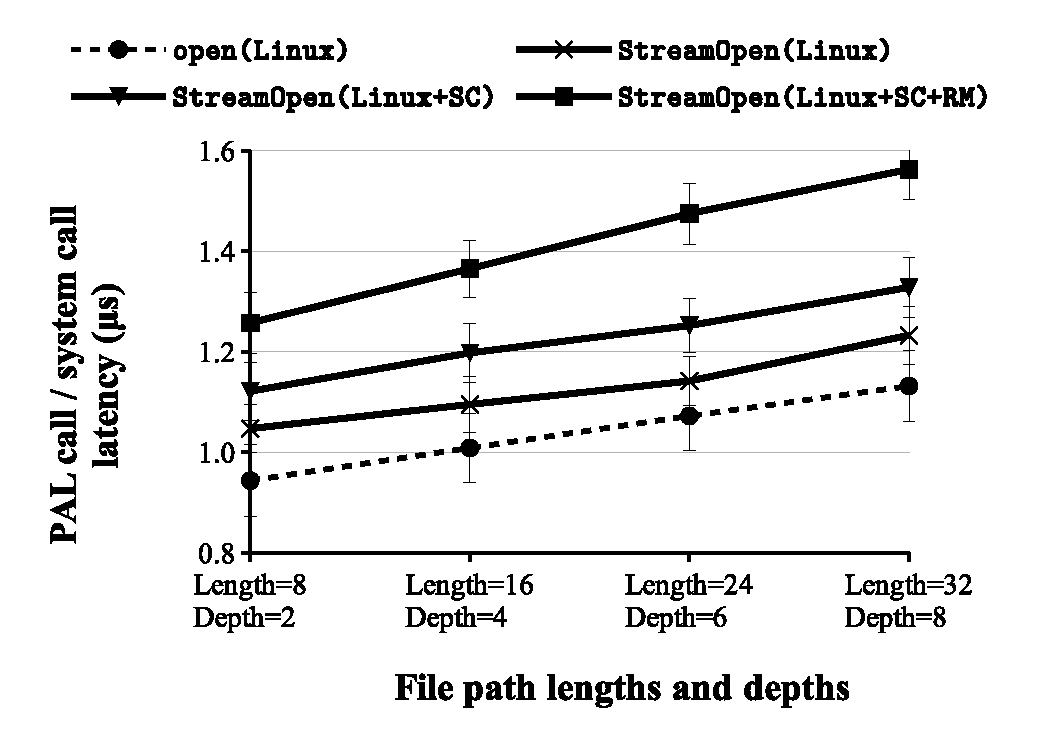
\includegraphics[width=24em]{pal-open-latency}\\
{\bf (a) Linux vs. Linux PAL}
\vspace{6pt}
\end{minipage}
\begin{minipage}{.49\linewidth}
\centering
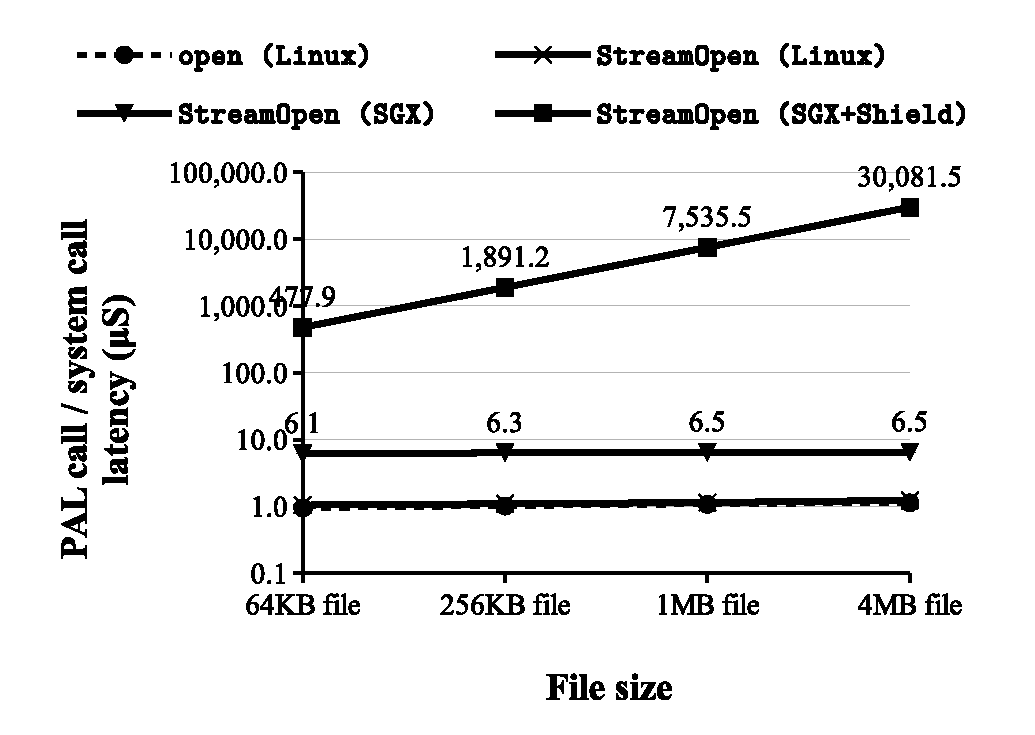
\includegraphics[width=24em]{sgx-open-latency}\\
{\bf (b) Linux vs. Linux PAL vs. SGX PAL}
\vspace{6pt}
\end{minipage}
\caption{Latency of \palcall{StreamOpen} on Linux and SGX, and \syscall{open} \linuxapis{} in a native Linux process. Figure (a) shows the comparison between \syscall{open} \linuxapis{} and \palcall{StreamOpen} on a Linux PAL,
with the options of enabling the SECCOMP filter ({\bf +SC})
and reference monitor ({\bf +RM}). Figure(b) shows the comparison between  \syscall{open} \linuxapis{}, \palcall{StreamOpen} on a Linux PAL,
and \palcall{StreamOpen} inside an SGX enclave, either with or without
integrity protection ({\bf +Shield}).}
\label{fig:eval:pal:open-latency}
\end{figure*}


Figure~\ref{fig:eval:pal:open-latency} (b) shows the latency of \palcall{StreamOpen} inside of an SGX enclave, versus the latency of 
\palcall{StreamOpen} and \syscall{open} on Linux.
Without security checks to shield an enclave from the OS,
the latency of \palcall{StreamOpen} is dominated by the overhead of exiting the enclave and copying the argument out of the enclave,
for accessing the host \linuxapis{}.
The overheads of unshielded \palcall{StreamOpen} is 4.7--5.5$\times$, or \roughly{}5 \msec{}.
If a file is shielded with integrity protection,
\palcall{StreamOpen} will verify the checksum of the whole file against the manifest, and generate a Merkel Tree of file chunk hashes
for optimizing the latency of following \palcall{StreamRead} or \palcall{StreamMap}.
The overhead of enforcing the integrity check is correlated with the file size, and dominated by the time of
calculating a SHA256 hash of the file.
For a 4MB file, the latency of \palcall{StreamOpen} can be up to \roughly{}30 milliseconds.



\paragraph{File reads and writes.}


\begin{figure*}[t!]
\centering
\footnotesize
\begin{minipage}{.49\linewidth}
\centering
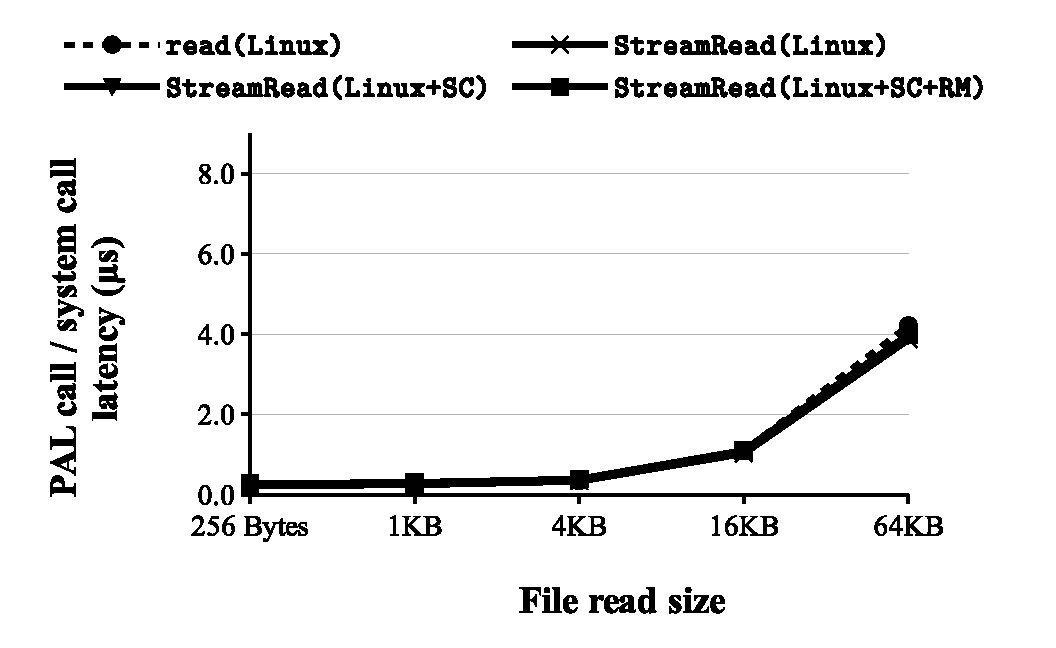
\includegraphics[width=24em]{pal-read-latency}\\
{\bf (a) Sequential read}
\vspace{6pt}
\end{minipage}
\begin{minipage}{.49\linewidth}
\centering
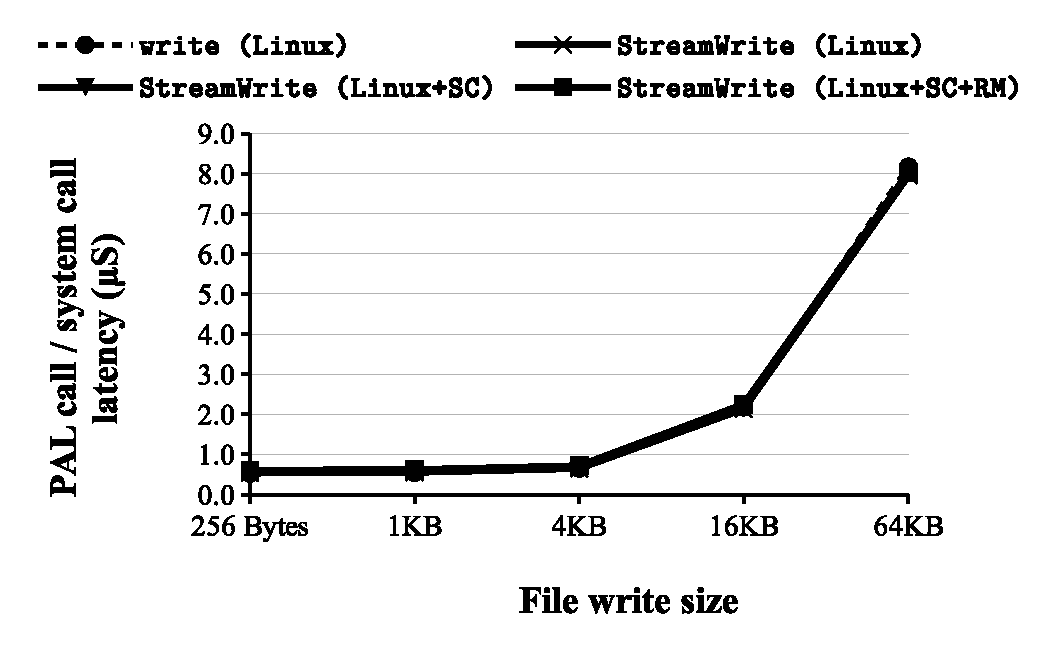
\includegraphics[width=24em]{pal-write-latency}\\
{\bf (b) Sequential write}
\vspace{6pt}
\end{minipage}
\caption{Latency of sequential \palcall{StreamRead} and \palcall{StreamWrite} on Linux, compared with the latency of \syscall{read} and \syscall{write} \linuxapis{} in a native Linux process. The comparison is between the \linuxapis{} and the \hostapis{} on a Linux PAL,
with the options of enabling the SECCOMP filter ({\bf +SC})
and reference monitor ({\bf +RM}).}
\label{fig:eval:pal:read-write-latency}
\end{figure*}

\begin{figure*}[t!]
\centering
\footnotesize
\begin{minipage}{.49\linewidth}
\centering
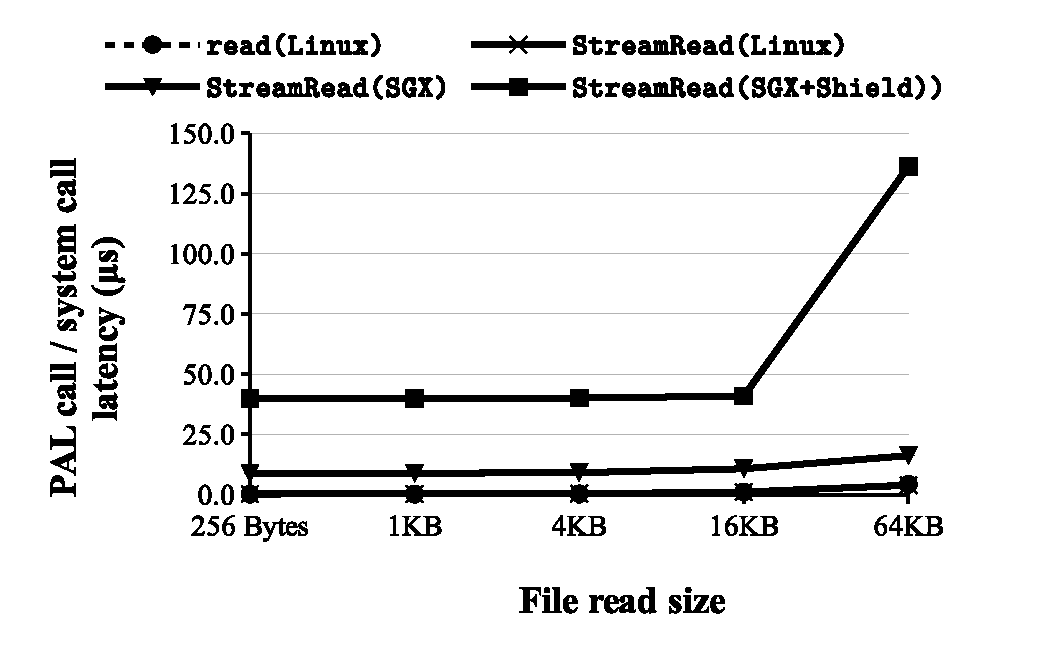
\includegraphics[width=24em]{sgx-read-latency}\\
{\bf (a) Sequential read}
\vspace{6pt}
\end{minipage}
\begin{minipage}{.49\linewidth}
\centering
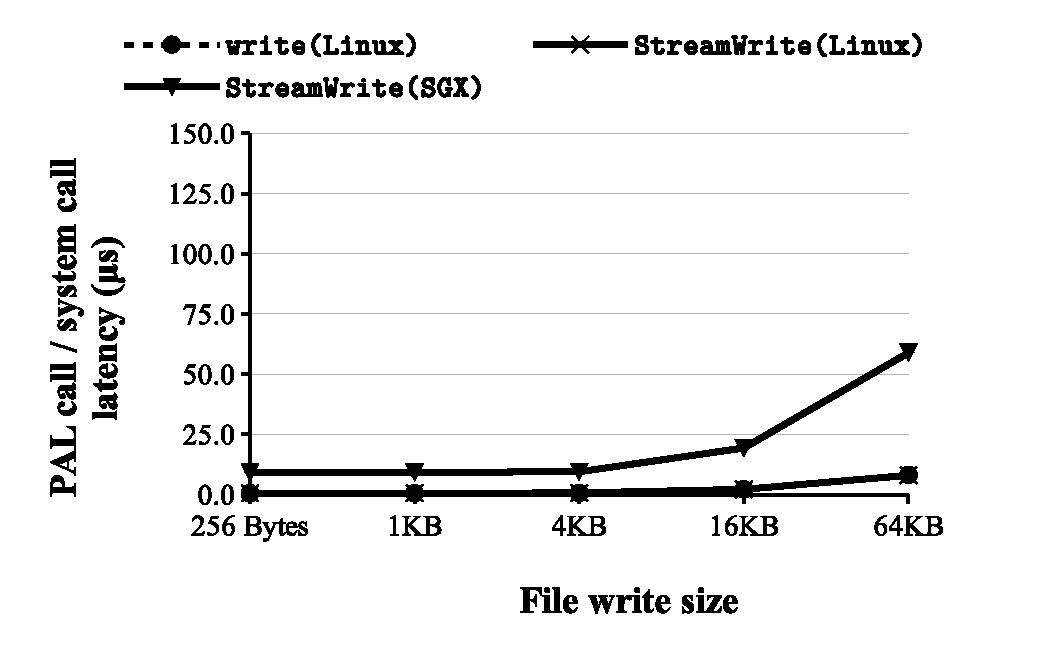
\includegraphics[width=24em]{sgx-write-latency}\\
{\bf (b) Sequential write}
\vspace{6pt}
\end{minipage}
\caption{Latency of sequential \palcall{StreamRead} and \palcall{StreamWrite} inside an SGX enclave, compared with the latency of \syscall{read} and \syscall{write} \linuxapis{} in a native Linux process. The comparison is between (1) \linuxapis{}; (2) \hostapis{} on a Linux PAL (without the SECCOMP filter and reference monitor); (3) \hostapis{} in an enclave, either with or without integrity protection ({\bf +Shield}).
The integrity protection for contents written by \palcall{StreamWrite}
is left as future work.}
\label{fig:eval:pal:sgx-read-write-latency}
\end{figure*}


\paragraph{Network connections.}



\paragraph{Network latency and bandwidth.}



\paragraph{RPC latency and bandwidth.}







\subsection{Paging and exception handling}























\subsection{Scheduling}
















\subsection{Multi-process abstractions}













\subsection{Miscellaneous}

